\documentclass{article}
% ----- Preamble
\usepackage[utf8]{inputenc} % police encodee en latin1=iso8859-1=Windows Latin 1 %
\usepackage[french]{babel} % police fr %
\usepackage{hyperref} % pour les references %
\usepackage{amsmath} % pour les formules de maths %
\usepackage{amssymb} % pour les symboles maths %
\usepackage{amsthm} % pour la mise en forme des theoremes %
\usepackage{aeguill} % pour les guillemets et accents francais %
\usepackage{listings} % pour les listings de code %
\usepackage{helvet} % police helvetica %
\usepackage{graphicx}
\usepackage{centernot}
\usepackage{dsfont}
\usepackage{subcaption}
\usepackage{caption}
% modification des dimensions de la page et de son centrage %
\topmargin 0.0cm
\oddsidemargin 0.1cm
\textwidth 16cm 
\textheight 22cm
\footskip 0.0cm

\title{Traitement d'Image et du Signal - TP6}
\author{Laurent Cetinsoy, Karim Kouki, Aris Tritas }
\date{\today}

\begin{document}
\maketitle

\section{Echange de phase}

Dans cette partie on s'intéresse à l'information portée par la phase et le module de la TFD d'une image. 


\begin{figure}[h]
	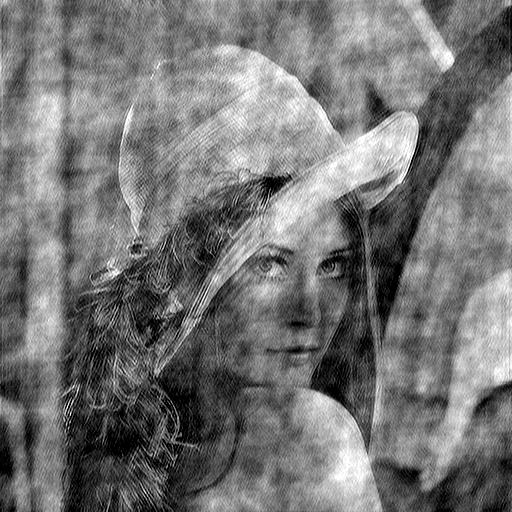
\includegraphics[width=0.5\textwidth]{phase_swapping.jpg}
	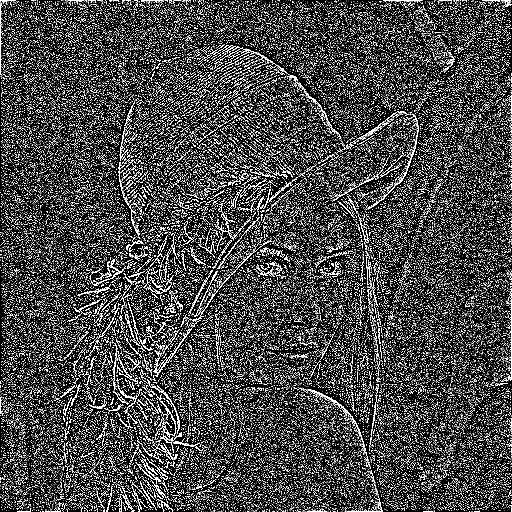
\includegraphics[width=0.5\textwidth]{phase_swapping_in_random.jpg}
	\newline
	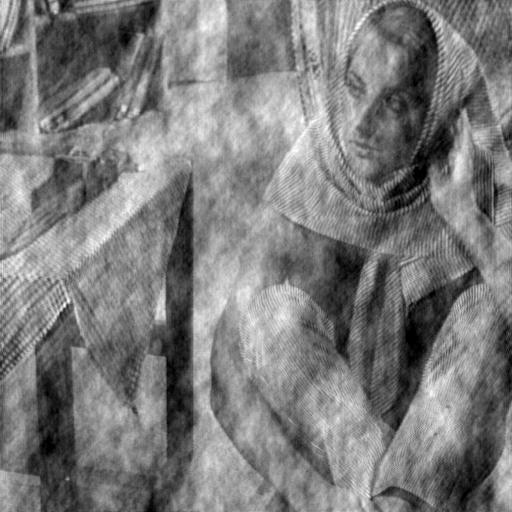
\includegraphics[width=0.5\textwidth]{module_swapping.jpg}

  \caption{A gauche l'image originale et l'histogramme correspondant. A droite l'image dont l'histogramme a été égalisé. }
\end{figure}


On constate qu'une grande partie de l'information est portée par la phase. Il est aussi intéressant de notée qu'elle a besoin de variation pour s'exprimer. 

Inversement le module de la TFD ne porte que peu d'information. 


\end{document}